% Chapter Template

\chapter{Introduction} % Main chapter title
\label{Chapter1}
As part of my Bachelor degree, I did an internship for three months in Beat, a company that started as a Greek startup about 5 years ago. From March 18th 2019 until June 18th 2019, I contributed as a Software Developer intern in several projects that was referred to a product named "BeatHotels".

\section{Company Description}
%βασικά χαρακτηριστικά κύριες δραστηριότητες
Beat is a company that is developing a mobile application for taxi cab and peer-to-peer-ridesharing. The app is based on the idea of establishing a direct connection between drivers and passengers by offering both sides a modern alternative to conventional booking processes. First known as a greek startup named Taxibeat, the company was founded in 2011 by Nikos Drandakis in collaboration with associates Kostis Sakkas, Nikos Damilakis and Michael Sfictos. Taxibeat was acquired in February 2017 by MyTaxi, a subsidiary of the automotive manufacturer Daimler AG, and renamed to Beat. Nowadays, Beat is part of the FreeNow group and its CEO is Nikos Drandakis. The FreeNow group is the ride hailing joint venture from Daimler and BMW, and consists of the services MyTaxi, Beat, Kapten, Clever and Hive, the e-Scooter service. \par % Diagram

\begin{figure}[h!]
	\begin{center}
		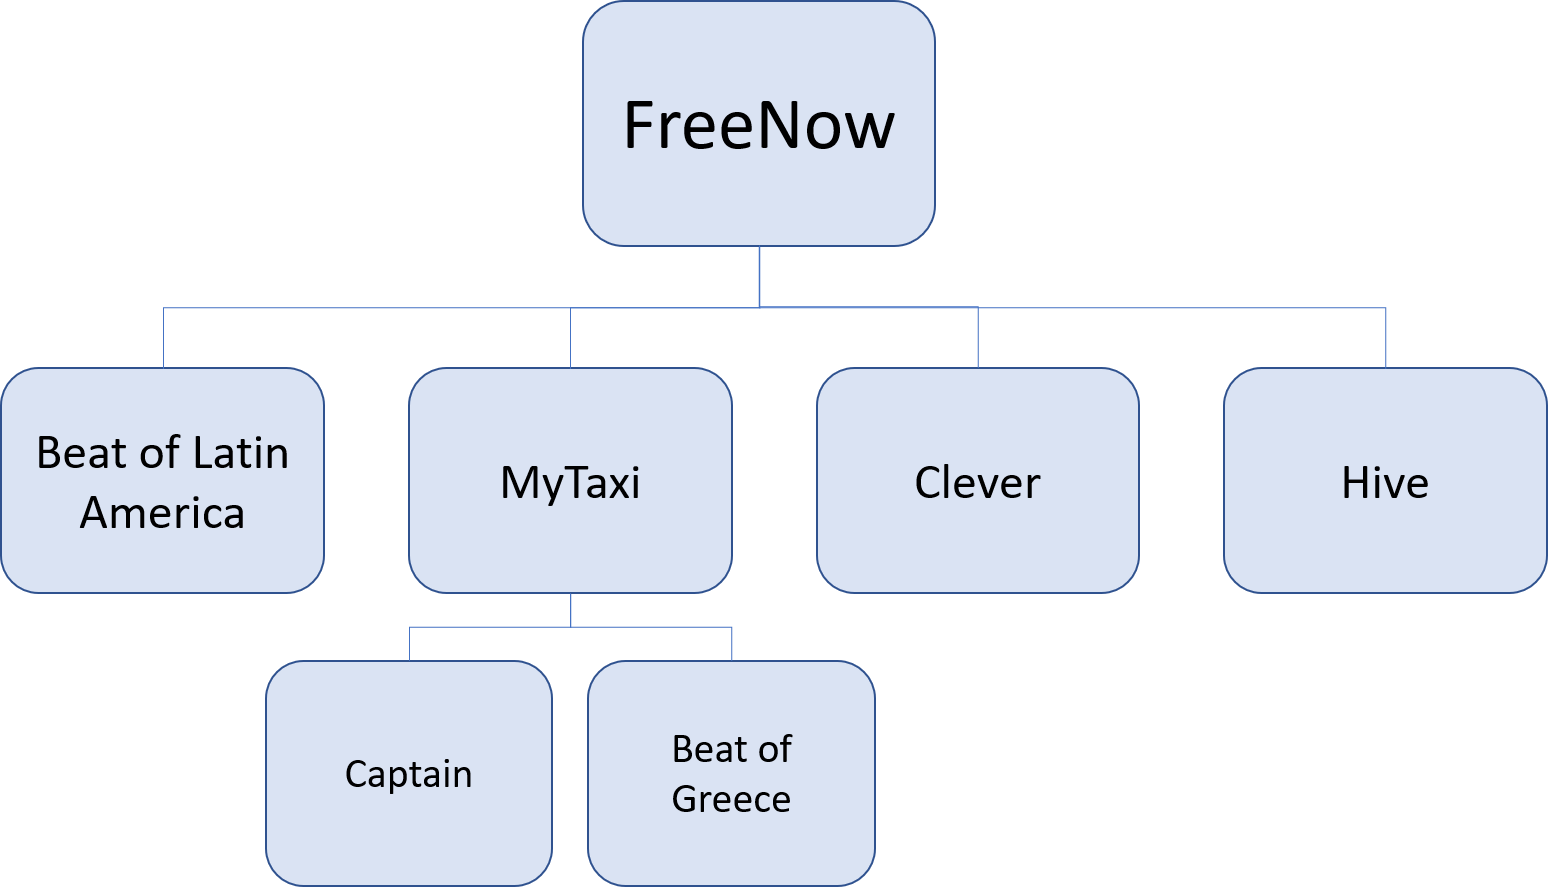
\includegraphics[scale=0.5]{images/FreeNow_structure.png}
	\end{center}
	\caption{FreeNow's structure}
\end{figure}
\newpage

Beat headquarters in Athens, Greece, while additional development and operation offices are located in Lima, Santiago, Cali, Medellín, Bogotá and Mexico City. It currently has more than 580 employees all over the world, with approximately 400 of them being in Greece. Company's teams work in small, autonomous groups of people following agile methodologies. \par
As regards Beat's structure, it is slightly different after its buyout. More specifically, the firm is separated in two parts based on its market targets, Beat of Latin America and Beat of Greece. This separation is because Greek market is basically part of MyTaxi group, while Latin America Market is only part of FreeNow, as shown at the driagram above. So, Beat has eight main departments, Business Operations, Finance, Engineering, Greek Market, People Operations, Marketing, Operating Office and Senior Management Team. The last department mentioned is conducted by Nikos Drandakis and his team as picture bellow reveals.\par
\begin{figure}[h!]
	\begin{center}
		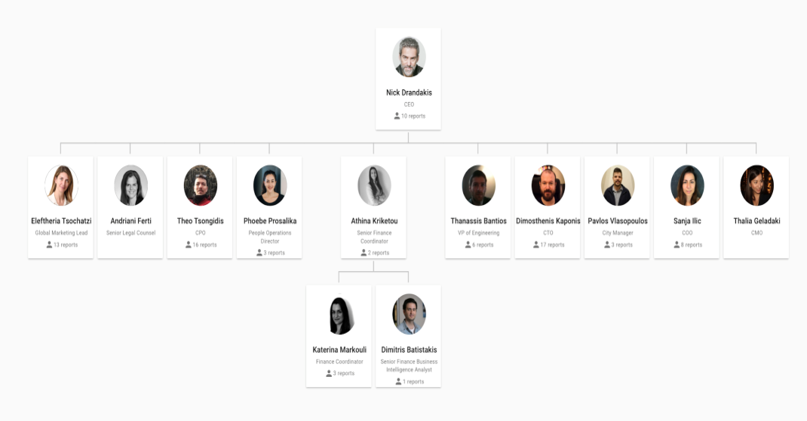
\includegraphics[scale=0.7]{images/organization.png}
	\end{center}
	\caption{Beat's SMT Department}
\end{figure}
Products provided by Beat are mainly three in number. Beat App, with the extended service of peer-to-peer-ridesharing in Latin America Marketplace, Beat Hotels, B2B service only provided in Greece, and Hive, e-scooter services in Greek Market.\par

\subsection{Beat App}
Beat App is a B2C service provided in both Androids and IOS operating systems.
\begin{wrapfigure}[9]{r}{0.3\textwidth}
	\begin{center}
		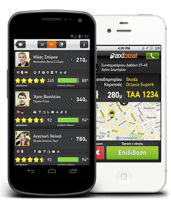
\includegraphics[scale=0.7]{images/beat_app.png}
	\end{center}
	\caption{Beat App}
\end{wrapfigure}
This service is a connection between drivers and candidate passengers.\par 
In other words, someone looking for a cup can find the closest one without any extra costs by using passenger's Beat app. Anyone that has downloaded the app can call a cup from any place, be able to see driver's rating from other Beat passengers, their personal data such as name, plates and more car details or services provided. In addition, before ride starts, an estimated price is given, list of the closest drivers is shown, and the candidate passenger has the ability to choose one of them based on the details and services provided, and to rate when ride is completed. \par
On the other hand, driver use another app through which the connection between two-sides is succeed. Available drivers can be located and the closest ones are shown to the candidate passenger. Driver can also accept or reject a ride, see the recommended route and see where passenger is before departure.

\subsection{Beat Hotels}
Beat Hotels is a B2B service that has the same aim with Beat App, the connection between candidate passengers, in this case people staying in a Hotel and request 
\begin{wrapfigure}[12]{r}{0.3\textwidth}
	\begin{center}
		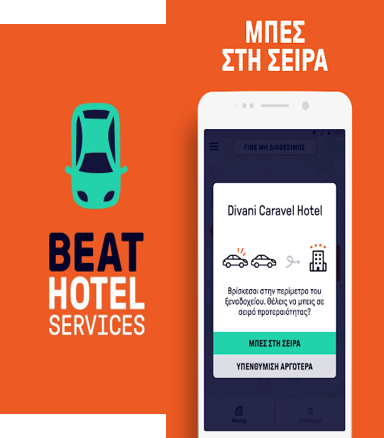
\includegraphics[scale=0.5]{images/beat_hotels.png}
	\end{center}
	\caption{Beat Hotels}
\end{wrapfigure}
for a taxi, and drivers.
The difference between these two services is, except from the aimed passengers, the virtual queues of drivers created in each Hotel.\par
There is a driver app, different from Beat driver's app, created in React Native and Node.js. This app is used from the driver in order to check the available Hotel queues and how much complete they are, get in a queue and start a ride.\par
On the other side, Hotel's have a customized dashboard, written in ReactJs and Node.js. Through this dashboard, they can call a taxi for a customer, see where the taxi is any time and get statistics of rides and revenue they have from rides completed.\par
Finally, a similar dashboard is developed for the agents of Beat with all the informations of each Hotel that Beat's corporate. The agents have the permissions also to change the amount of a ride if it is needed, check all completed rides, or block a driver with inappropriate behavior.

\subsection{Hive}
Hive is an e-scooter sharing system service. Scooters are made available to use for short-term rentals and can be dropped off or picked up from arbitrary 
\begin{wrapfigure}[8]{r}{0.2\textwidth}
	\begin{center}
		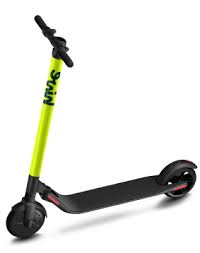
\includegraphics[scale=0.2]{images/hive.png}
	\end{center}
	\caption{Hive}
\end{wrapfigure}
locations in the service area.
Hive has an app through which a candidate user, can find where e-scooters are in the map, how much battery they have and their cost, scan the barcode of the e-scooter, unlock and rent it. \par 
However, as regards Beat's part in Hive service is limited. Beat only provide customer experience services by receiving e-mails from users and resolving their issues occurred either from e-scooters or the app. Beat also is responsible of placing the e-scooters in the right places and charge them.

\newpage
\section{Internship Goal}
 As regards internship's goal, is to gain experience as a Software Developer, learning tools like React, Redux and Node.js, understanding how an application works in production. Learning how to code in Javascript and improving a web site for BeatHotel's agents by completing tasks given, and creating npm packages, were my main responsibilities as an intern.
 
\section{Report's Structure}
The internship's report is an overview of what I have been interacted with during my internship, analyzing the projects and results, skills that I have gained or used, and my role as an intern in general.

% 5 pages